% =============================================================================
% SENTINEL — Capstone Project Proposal (LaTeX)
% Template: FPT University MSE Proposal Format
% Author: Nguyễn Đức Bình
% =============================================================================
\documentclass[12pt,a4paper]{article}

% --- Packages ---
\usepackage[utf8]{inputenc}
\usepackage[T5]{fontenc}
\usepackage[english]{babel}
\usepackage{times}
\usepackage{geometry}
\geometry{left=3cm, right=2.5cm, top=2.5cm, bottom=2.5cm}
\usepackage{graphicx}
\usepackage{tikz}
\usetikzlibrary{shapes.geometric, arrows.meta, positioning, fit, backgrounds}
\usepackage{pgfgantt}
\usepackage{hyperref}
\usepackage{booktabs}
\usepackage{enumitem}
\usepackage{amsmath}
\usepackage{amssymb}
\usepackage{url}
\usepackage{cite} % IEEE numbered citation style
\usepackage{array}
\usepackage{longtable}
\usepackage{float}
\usepackage{setspace}
\usepackage{titlesec}
\usepackage{fancyhdr}
\usepackage{listings}
\usepackage{xcolor}

\lstset{
    basicstyle=\ttfamily\small,
    breaklines=true,
    frame=single,
    backgroundcolor=\color{gray!5},
    keywordstyle=\color{blue},
    commentstyle=\color{green!60!black},
    stringstyle=\color{orange},
    showstringspaces=false,
    inputencoding=utf8,
    extendedchars=true
}

% --- Formatting ---
\setstretch{1.3}
\setlength{\parskip}{6pt}
\setlength{\parindent}{0pt}

\hypersetup{
    colorlinks=true,
    linkcolor=blue,
    citecolor=blue,
    urlcolor=blue,
}

\titleformat{\section}{\large\bfseries}{\thesection.}{0.5em}{}
\titleformat{\subsection}{\normalsize\bfseries}{\thesubsection}{0.5em}{}

\pagestyle{fancy}
\fancyhf{}
\fancyfoot[C]{\thepage}
\renewcommand{\headrulewidth}{0pt}

% =============================================================================
\begin{document}

% --- COVER PAGE ---
\begin{titlepage}
    \centering

    \vspace*{1cm}
    {\large\textbf{FPT University}}\\[0.5cm]
    {\normalsize Graduate School of Information Technology}\\[2cm]

    \rule{\textwidth}{0.5pt}\\[0.5cm]
    {\LARGE\textbf{A Cognitive Two-Tier Architecture for\\Automated Threat Detection and\\Contextual Response using Agentic AI}}\\[0.5cm]
    \rule{\textwidth}{0.5pt}\\[1cm]

    {\large\textit{Capstone Project Proposal}}\\[2cm]

    \begin{tabular}{rl}
        \textbf{Author:}     & Nguyễn Đức Bình \\
        \textbf{ID:}         & MSE13183        \\[0.5cm]
        \textbf{Supervisor:} & Bùi Văn Hiệu    \\
    \end{tabular}

    \vfill
    {\normalsize Hanoi, 2026}

\end{titlepage}

% --- ABSTRACT ---
\newpage
\addcontentsline{toc}{section}{Abstract}
\section*{Abstract}
In modern cybersecurity, Security Operations Centers (SOCs) face a critical ``Big Data Paradox'': an overwhelming volume of security events per second leads to severe alert fatigue. Traditional IDS and SIEM platforms analyze data in isolation, reducing the capability to detect sophisticated multi-stage Advanced Persistent Threats (APTs). While Large Language Models (LLMs) and Agentic AI offer automated triage, their deployment exposes organizations to two fatal flaws: excessive reasoning latency incompatible with wire-speed packet processing, and vulnerability to adversarial log-substrate prompt injection attacks.

To address these limitations, this study proposes a self-defending cognitive two-tier architecture named SENTINEL. Tier 1 filters benign traffic and scans for unsupervised anomalies using an $O(1)$ online Welford statistical engine at wire speed (reducing overall latency by $99.9\%$ with local triage in $0.6$\,ms). Tier 2 acts as a stateful LangGraph agent running a local quantized Gemma-2-9B-IT model (GGUF Q6\_K format) via llama.cpp. To ground reasoning, Tier 2 employs a Dual-RAG search engine combining FAISS dense vector search and BM25 sparse keyword matching integrated via Reciprocal Rank Fusion (RRF). Security guardrails include a Delimited Data Encapsulation layer to neutralize injections, an in-memory LRU semantic cache with SHA-256 keys, and HMAC signatures for audit trail integrity.

Evaluated on the CSE-CIC-IDS2018 and DAPT2020 datasets, the system demonstrates robust zero-day anomaly detection ($7/7$) and absolute APT recall ($1.0$). A cross-family LLM-as-a-Judge evaluation using Llama-3-8B-Instruct scores the RAGAS context quality at $3.91/5$ (Faithfulness at $4.00/5$), while the static guardrails successfully block $50.0\%$ of adversarial payloads (neutralizing $100\%$ of encoding-bypasses) and route semantic confusion to a Human-in-the-Loop (HITL) queue, establishing a secure, scalable automation standard for modern SOCs.

% --- TABLE OF CONTENTS ---
\newpage
\tableofcontents

% =============================================================================
% CHAPTER 1: INTRODUCTION AND BACKGROUND
% =============================================================================
\newpage
\section{Introduction and Background}

\subsection{Research Problem}
Modern Security Operations Centers (SOCs) are overwhelmed by the sheer volume of security events. According to recent industry reports, the average SOC analyst processes thousands of alerts daily, with nearly half identified as false positives \cite{ponemon2023}. This phenomenon, known as \textit{alert fatigue}, leads to critical threats being overlooked. Traditional IDS/SIEM systems exacerbate this problem by analyzing data sources (Web logs, Firewall logs, Authentication logs) in isolation, severely reducing the ability to detect sophisticated multi-stage attack chains such as Advanced Persistent Threats (APTs).

The application of Large Language Models (LLMs), particularly Agentic AI and Retrieval-Augmented Generation (RAG) architectures, to automated log analysis introduces critical operational and security vulnerabilities. First, the \textit{reasoning latency} is prohibitively high for real-time streaming environments. Second, Agentic AI architectures drastically expand the attack surface beyond traditional LLMs. These autonomous systems are highly susceptible to a spectrum of adversarial vectors: \textit{Indirect Prompt Injection} and \textit{Jailbreaks} hidden within log data \cite{greshake2023}, where adversaries embed malicious instructions in dynamic fields (e.g., User-Agent) to hijack the agent's logic. Furthermore, granting agents access to execution environments creates the risk of \textit{Sandbox Escape} and \textit{Remote Code Execution (RCE)}, while rendering LLM outputs on analyst dashboards introduces \textit{Data Exfiltration} vulnerabilities via malicious Markdown rendering. Additionally, relying on external knowledge bases exposes the system to \textit{RAG Poisoning}, where threat actors manipulate reference documents to subvert the agent's contextual understanding. This creates a fundamental paradox: analysts must grant the agent dynamic context and execution capabilities to analyze attacks, yet doing so exposes the SOC infrastructure to hijacking. Under a Zero Trust Architecture (ZTA) framework \cite{nist80207}, all autonomous actions must be continuously authenticated, authorized, and verified, rather than implicitly trusted.

\subsection{Research Objectives}
Motivated by these limitations, this study aims to develop an autonomous AI Security Agent utilizing a cognitive two-tier architecture. Instead of relying purely on a single LLM to process all logs, the thesis proposes a hybrid approach: a high-speed deterministic rule engine combined with a deep-reasoning LLM Agent. This approach is expected to drastically reduce reasoning latency by filtering noise, mitigate prompt injection via bounded encapsulation, and enhance context awareness using Long-Term Threat Memory and a Dual-RAG setup (incorporating MITRE ATT\&CK for tactical threat identification and NIST SP 800-61r2 for incident response guidance). A Human-in-the-Loop (HITL) Web Dashboard will also be developed to demonstrate practical SOC automation.

\subsection{Research Questions}
Based on the objectives, this thesis focuses on four core research questions:
1. Does a Two-Tier Architecture (Rule-based + LLM Agent) combined with Session-Aware Behavioral Baselining and unsupervised online Welford anomaly detection optimize Reasoning Latency compared to a One-Tier (LLM-only) approach?
2. Can a Delimited Data Encapsulation mechanism (using Dynamic Randomized Delimiters) effectively prevent structural Prompt Injections (e.g., Delimiter Smuggling) without degrading the LLM's classification accuracy?
3. How does a Dual-RAG pipeline (combining tactical threat frameworks with incident response standards) improve the Context Relevance of the LLM's threat analysis?
4. Can an adaptive Feedback Loop with HITL Quarantine and Few-shot Active Learning prevent Adversarial Rule Injection and safely automate defensive responses?

\subsection{Research Object and Methodology}
The primary objects of this research are the Two-Tier Security Architecture, Agentic AI (LLMs applied to SOC automation), Adversarial Prompt Injections, and network intrusion log data.
The study employs a Quantitative Experimental methodology, utilizing an Ablation Study to compare the Two-Tier system against a baseline LLM-only setup. Evaluation is conducted using a 5-Dimensional (5D) Framework covering Classification metrics, Operational latency, Adversarial Robustness, RAGAS-based Context Quality (via cross-family LLM-as-a-Judge), and Explainability.

\subsection{Scope of the Study}
The research is limited to Network Intrusion Detection and SOC log triage. The in-scope components include: Data Streaming Pipeline (Redis), Tier-1 Rule Engine, LangGraph Agent with Dual-RAG, Guardrails (Volume Compression and Injection Defense), and a Streamlit HITL Dashboard with SQLite-based Threat Memory. The study does not cover fine-tuning Foundation Models, physical hardware deployment (e.g., physical Kafka clusters), or Layer 3/4 volumetric DDoS mitigation.

\subsection{Thesis Structure}
The thesis will be organized into six main chapters: (1) Introduction and Background; (2) Literature Review; (3) Proposed Solution and Research Methodology; (4) Implementation and Evaluation Plan; (5) Expected Results and Contributions; and (6) Conclusion.

% =============================================================================
% CHAPTER 2: LITERATURE REVIEW
% =============================================================================
\newpage
\section{Literature Review}

\subsection{Foundational Approaches}
In the early stages of network security, Intrusion Detection Systems (IDS) primarily relied on signature-based matching (e.g., Snort, Suricata) to detect known threats. While highly efficient in terms of throughput, these systems exhibit significant limitations in identifying zero-day attacks and polymorphic malware \cite{khraisat2019}.

The advent of Machine Learning (ML) led to anomaly-based IDS, where models such as Random Forests, LSTMs, and domain-specific transformers like LogBERT \cite{logbert2021} learn a baseline of normal behavior and flag deviations. While these approaches improved zero-day detection, they remain fundamentally limited to pattern-based anomaly scoring. They cannot explain \textit{why} a log sequence is malicious, map threats to standardized frameworks, or generate actionable remediation steps—capabilities that require the contextual reasoning of a Large Language Model. These pattern-based models, by design, cannot query external knowledge bases at inference time---a fundamental architectural constraint that precludes contextual threat mapping and actionable remediation.

Modern Security Information and Event Management (SIEM) systems aggregate logs, yet they still require extensive manual triage by human analysts to construct the full context of an attack.

\subsection{Related Work}
The recent emergence of Large Language Models (LLMs) has opened new directions for automated log summarization and incident response. Comprehensive surveys such as \cite{habibzadeh2025} demonstrate the growing adoption of cloud-based LLM APIs (e.g., GPT-4) for SOC automation, including log summarization and incident triage. However, relying on cloud APIs violates strict organizational data privacy policies and introduces unacceptable network latency for real-time triage.

In the realm of knowledge-augmented threat analysis, knowledge graph-based approaches to threat intelligence mapping \cite{attackg2023} have shown promising results in automatically extracting and structuring attack techniques from CTI reports into MITRE ATT\&CK-aligned graphs. Yet, existing studies generally focus solely on tactical analysis, lacking the integration of operational incident response standards (such as NIST SP 800-61r2) required for actionable SOC remediation.

Regarding adversarial robustness, the OWASP Top 10 for LLM Applications \cite{owasp2025} and the Agent Security Bench (ASB) \cite{zhang2024asb} highlight that LLM agents suffer from high attack success rates via prompt injection. While the Drain3 algorithm \cite{he2017} is widely used for log template mining, it is typically employed for storage compression rather than active injection defense. Furthermore, recent methodologies for LLM evaluation emphasize the need to address Self-Enhancement Bias by employing cross-family evaluation or statistical validation instead of isolated LLM-as-a-Judge paradigms \cite{zheng2023, ragas2023}. These studies reveal a critical research gap that this thesis seeks to address: the absence of a unified, self-defending architecture with rigorous, multi-dimensional evaluation.

\subsubsection{Comparative Analysis of Existing Approaches}

\begin{table}[H]
    \centering
    \caption{Comparison of approaches for SOC log analysis}
    \label{tab:comparison}
    \begin{tabular}{lccccc}
        \toprule
        \textbf{Approach}                   & \textbf{Local} & \textbf{Real-time} & \textbf{Anti-Injection} & \textbf{RAG} & \textbf{HITL} \\
        \midrule
        Signature IDS (Snort)               & \checkmark     & \checkmark         & N/A                     & --           & --            \\
        ML Anomaly IDS (RF/LSTM)            & \checkmark     & \checkmark         & --                      & --           & --            \\
        LogBERT \cite{logbert2021}          & \checkmark     & \checkmark         & --                      & --           & --            \\
        Cloud LLM SOC \cite{habibzadeh2025} & --             & --                 & --                      & Partial      & --            \\
        \textbf{SENTINEL (Ours)}            & \checkmark     & \checkmark         & \checkmark              & \checkmark   & \checkmark    \\
        \bottomrule
    \end{tabular}
\end{table}

% =============================================================================
% CHAPTER 3: PROPOSED SOLUTION AND RESEARCH METHODOLOGY
% =============================================================================
\newpage
\section{Proposed Solution and Research Methodology}

\subsection{Proposed Solution: Cognitive Two-Tier Architecture}
The proposed solution is based on a cognitive Two-Tier Architecture designed with a strict Separation of Concerns. The core idea is to leverage the speed of deterministic rules (Tier 1) alongside the deep reasoning capabilities of an Agentic LLM (Tier 2), interconnected by robust adversarial guardrails.

\begin{figure}[H]
    \centering
    \resizebox{\textwidth}{!}{
    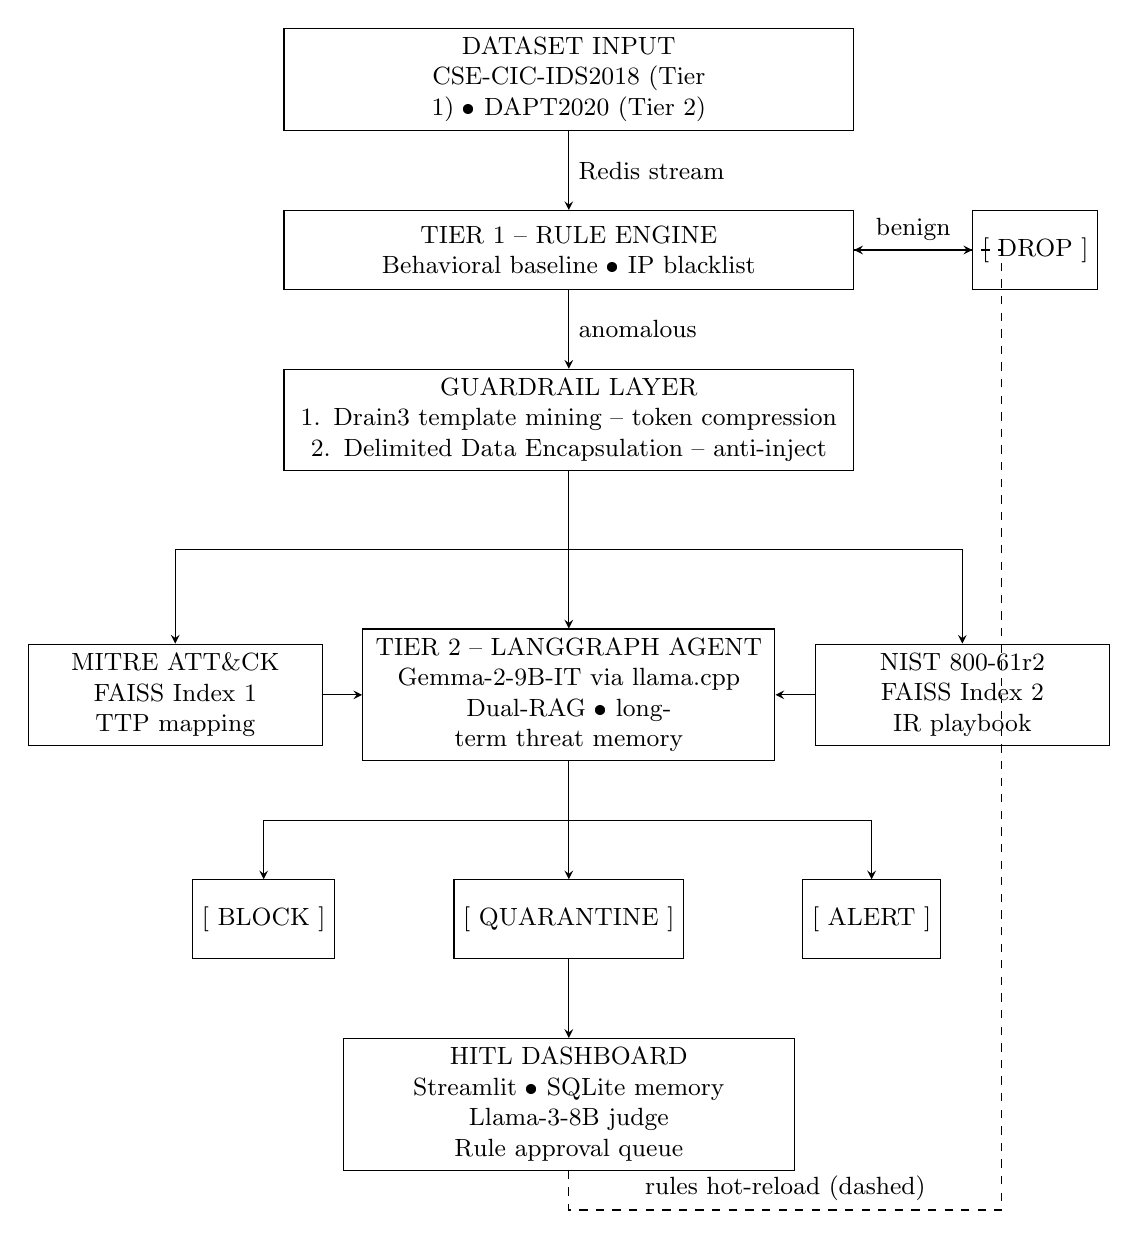
\begin{tikzpicture}[
        >=stealth,
        node distance=1cm and 0.5cm,
        font=\small,
        box/.style={draw, rectangle, minimum height=1cm, align=center, fill=white},
    ]

    % Nodes
    \node[box, text width=7cm] (dataset) {DATASET INPUT \\ CSE-CIC-IDS2018 (Tier 1) \textbullet\ DAPT2020 (Tier 2)};
    \node[box, text width=7cm, below=1cm of dataset] (tier1) {TIER 1 -- RULE ENGINE \\ Behavioral baseline \textbullet\ IP blacklist};
    \node[box, right=1.5cm of tier1] (drop) {[ DROP ]};

    \node[box, text width=7cm, below=1cm of tier1] (guardrail) {GUARDRAIL LAYER \\ 1. Drain3 template mining -- token compression \\ 2. Delimited Data Encapsulation -- anti-inject};

    \node[box, text width=5cm, below=2cm of guardrail] (tier2) {TIER 2 -- LANGGRAPH AGENT \\ Gemma-2-9B-IT via llama.cpp \\ Dual-RAG \textbullet\ long-term threat memory};
    \node[box, text width=3.5cm, left=0.5cm of tier2] (mitre) {MITRE ATT\&CK \\ FAISS Index 1 \\ TTP mapping};
    \node[box, text width=3.5cm, right=0.5cm of tier2] (nist) {NIST 800-61r2 \\ FAISS Index 2 \\ IR playbook};

    \node[box, below=1.5cm of tier2] (quarantine) {[ QUARANTINE ]};
    \node[box, left=1.5cm of quarantine] (block) {[ BLOCK ]};
    \node[box, right=1.5cm of quarantine] (alert) {[ ALERT ]};

    \node[box, text width=5.5cm, below=1cm of quarantine] (hitl) {HITL DASHBOARD \\ Streamlit \textbullet\ SQLite memory \\ Llama-3-8B judge \\ Rule approval queue};

    % Edges
    \draw[->] (dataset) -- node[right] {Redis stream} (tier1);
    \draw[->] (tier1) -- node[above] {benign} (drop);
    \draw[->] (tier1) -- node[right] {anomalous} (guardrail);

    % Routing from guardrail to MITRE/NIST and Tier 2
    \coordinate (split1) at ([yshift=-1cm]guardrail.south);
    \draw[-] (guardrail.south) -- (split1);
    \draw[->] (split1) -| (mitre.north);
    \draw[->] (split1) -| (nist.north);
    \draw[->] (split1) -- (tier2.north);

    \draw[->] (mitre.east) -- (tier2.west);
    \draw[->] (nist.west) -- (tier2.east);

    % Routing from tier2 to block/quar/alert
    \coordinate (split2) at ([yshift=-0.75cm]tier2.south);
    \draw[-] (tier2.south) -- (split2);
    \draw[->] (split2) -| (block.north);
    \draw[->] (split2) -| (alert.north);
    \draw[->] (split2) -- (quarantine.north);

    \draw[->] (quarantine) -- (hitl);

    \draw[->, dashed] (hitl.south) -- ++(0,-0.5) -| node[pos=0.25, above] {rules hot-reload (dashed)} ++(5.5,0) |- (tier1.east);

    \end{tikzpicture}
    }
    \caption{Cognitive Two-Tier Architecture}
    \label{fig:architecture}
\end{figure}

At the first stage, the Tier 1 Rule Engine acts as a heuristic filter. It maintains Session-Aware Behavioral Baselines using in-memory data structures (Redis) to track request rates and known malicious IPs. To proactively detect zero-day or signature-less anomalies, Tier 1 integrates an online Unsupervised Outlier Detector using Welford's algorithm to calculate the Running Mean and Standard Deviation ($O(1)$ time and memory complexity) of core network flow statistics (e.g., Flow Duration, Fwd/Bwd Packets, Fwd/Bwd Length). When a flow's Z-score exceeds the threshold ($|Z| > 3.5$), it is flagged as an Outlier Anomaly and escalated directly to Tier 2 for agentic investigation. This layer is designed to filter the majority of benign or purely volumetric noise at wire speed---filtering roughly 99.8\% of benign events and reducing average processing latency by over 99.9\% for Tier-1-resolved traffic---ensuring the downstream LLM is not overwhelmed by high-volume traffic.

Logs that exhibit anomalous behavior or trigger ambiguous thresholds are passed to the Guardrail Layer. Here, a two-step neutralization occurs:
1. \textbf{Template Mining (Drain3):} Extracts the static log template to compress the token volume without altering the dynamic payload variables.
2. \textbf{Delimited Data Encapsulation:} Dynamic payload fields are wrapped within cryptographically generated randomized delimiters (e.g., \verb|<<RANDOM_HEX>>|). This prevents adversaries from using Delimiter Smuggling to escape the data context and execute Prompt Injections.

Following the guardrails, the sanitized log enters Tier 2, governed by a LangGraph-based Agent. The Agent utilizes a Dual-RAG mechanism with two dedicated FAISS indexes, queried sequentially and merged before LLM inference:
\begin{itemize}
    \item \textbf{Index 1 — MITRE ATT\&CK:} Maps observed indicators to specific tactics, techniques, and procedures (TTPs), answering \textit{``what attack is happening?''}
    \item \textbf{Index 2 — NIST SP 800-61r2 \cite{nist80061}:} Retrieves the appropriate incident response phase (Preparation, Detection, Containment, Eradication, Recovery, Lessons Learned), answering \textit{``what should the SOC do next?''}
\end{itemize}
This fixed dual-index design eliminates the need for a routing mechanism, reducing failure points and ensuring predictable latency for evaluation. The separation bridges the gap between \textit{tactical identification} (MITRE: what happened) and \textit{operational response} (NIST: what to do about it).

To optimize classification and reasoning accuracy without resource-intensive offline fine-tuning, Tier 2 incorporates a Few-shot Active Learning feedback loop. The agent dynamically retrieves historical analyst approval (Approve) and rejection (Reject) decisions stored in system settings and structures them as prompt-level few-shot context. This allows the LLM to learn continuously from analyst feedback, avoiding repeat misclassifications.

Each index employs a \textbf{Hybrid Search} strategy combining dense semantic search (FAISS with \verb|all-MiniLM-L6-v2|) with sparse keyword matching (BM25Okapi), fused via \textbf{Reciprocal Rank Fusion (RRF, k=60)} \cite{rrf2009}. This dual-signal approach maximizes both semantic understanding and exact-match recall for security-specific identifiers such as CVE IDs, IP addresses, and port numbers. Retrieved chunks undergo \textbf{Structural Sanitization}---Unicode normalization, control character removal, and length truncation---to defend against RAG Poisoning before injection into the LLM prompt.

Finally, to ensure system safety against Adversarial Rule Injection, the LLM cannot directly modify the Tier 1 firewall. Instead, its recommended rules are placed into a Quarantine state (Human-in-the-Loop Feedback Loop). A SOC manager reviews these rules via a Dashboard before they are hot-reloaded into the Tier 1 engine.

\textbf{Short-Term and Long-Term SQLite Threat Memory:} The Tier 2 Agent relies on a persistent SQLite Threat Memory Store to correlate alerts across multi-day windows. When a new log is escalated, the system queries the IP's historical threat profile. If activities span multiple phases of the MITRE ATT\&CK matrix over time (e.g., Reconnaissance followed by Initial Compromise), the memory module dynamically escalates the threat severity level to critical, allowing for robust detection of slow-rate APT chains across the multi-day DAPT2020 campaigns (achieving full recall on the embedded APT actors in the evaluation stream).

\textbf{Human-in-the-Loop Web Dashboard (SOC UI):} A Streamlit interface with role-based access control (L1 Analyst and L3 Manager views) presents real-time alert queues, active firewall rules, a quarantine-management section, and a live False-Positive-Rate KPI derived from manual rule rejections. Analysts can click any IP to inspect its reputation score, AI-generated reasoning, and chronological event timeline, while administrators can hot-swap local LLM backends (e.g., Gemma-2-9B-IT and Llama-3-8B-Instruct) directly from the UI.

\textbf{Cryptographic Audit Trail with HMAC Validation:} To guarantee the integrity of security alerts and responses, the system implements a cryptographic audit trail stored in SQLite. Each log entry is cryptographically chained to the previous entry using a Keyed-Hash Message Authentication Code (HMAC-SHA256) \cite{hmac1997}. This prevents tampering or unauthorized deletion of event trails by adversaries who might compromise parts of the SOC dashboard, providing forensic-grade non-repudiation and integrity verification.

\textbf{Reproducibility:} MLflow logs all ablation metrics (classification scores, latencies, cache-hit and HITL escalation rates) across system configurations to ensure reproducible comparative analysis.

\subsection{Technologies and Tools}
The system is built on modern Python frameworks. The data streaming and short-term session tracking rely on Redis. The LLM reasoning engine utilizes a local quantized model (Gemma-2-9B-IT) in GGUF Q6\_K format, served via llama.cpp, ensuring absolute data privacy and full offline operation.

The agentic workflow is orchestrated by LangGraph, enabling cyclical decision-making and tool-use. For knowledge retrieval, \verb|sentence-transformers| is used alongside FAISS for dense semantic vector search and BM25Okapi (\verb|rank\_bm25|) for sparse keyword matching. The user interface and Human-in-the-Loop dashboard are developed using Streamlit, while long-term threat memory and audit trails are persisted using SQLite.

\subsubsection{Hardware Specification}
To ensure full reproducibility of latency benchmarks, all experiments are conducted on the following hardware:

\begin{table}[H]
    \centering
    \begin{tabular}{ll}
        \toprule
        \textbf{Component} & \textbf{Specification}                         \\
        \midrule
        CPU                & Intel Core i7-14700KF (28 threads) @ 5.700 GHz \\
        GPU                & NVIDIA GeForce RTX 4060 Ti (16 GB VRAM)        \\
        RAM                & 32 GB DDR5                                     \\
        OS                 & Ubuntu 24.04.4 LTS (x86\_64, Kernel 6.17)      \\
        LLM Backend        & llama.cpp with GGUF Q6\_K quantization          \\
        \bottomrule
    \end{tabular}
\end{table}

% =============================================================================
% CHAPTER 4: IMPLEMENTATION AND EVALUATION PLAN
% =============================================================================
\newpage
\section{Implementation and Evaluation Plan}

\subsection{Main Development Stages}
The implementation process will first focus on the Data Ingestion and Tier 1 Rule Engine. Two benchmark datasets are selected for evaluation:

\begin{itemize}
    \item \textbf{CSE-CIC-IDS2018 \cite{sharafaldin2018}:} The de facto standard for enterprise network intrusion detection research. As of 2025, no publicly available general-purpose enterprise NIDS dataset post-2018 exists. CIC's 2023--2026 releases (CICIoT2023, CIC-YNU-IoTMal 2026) target IoT environments and are not representative of enterprise SOC traffic. CSE-CIC-IDS2018 provides both raw PCAP and pre-extracted flow features, and its extensive adoption enables direct comparison with prior work.
    \item \textbf{DAPT2020 \cite{dapt2020}:} A purpose-built dataset for multi-stage Advanced Persistent Threat detection. This complements CSE-CIC-IDS2018 by providing attack chains that exercise SENTINEL's Tier 2 agent and Long-Term Threat Memory capabilities.
\end{itemize}

The session-tracking mechanism will be built using Redis TTLs to establish behavioral baselines.

Following this, the Guardrail Layer will be implemented, integrating the Drain3 algorithm for template mining and developing the cryptographic Delimited Data Encapsulation module to neutralize adversarial payloads.

The next critical step is the construction of the Tier 2 Agent using LangGraph and the Dual-RAG knowledge base. Two separate FAISS indexes will be populated: one with parsed MITRE ATT\&CK techniques and one with NIST SP 800-61r2 incident response procedures. The agent's prompts will be carefully engineered to strictly separate system instructions from the encapsulated payload data.

Finally, the Streamlit Dashboard and the SQLite Long-Term Threat Memory will be integrated. This phase will finalize the closed-loop process by enabling the Human-in-the-Loop feature, allowing administrators to approve dynamic rules generated by the LLM and feed them back to Tier 1.

\subsection{Evaluation Plan}
To validate the effectiveness of the system, the study employs a comprehensive 5-Dimensional (5D) Evaluation Framework.

To evaluate the system's baseline accuracy, an Ablation Study will be conducted. This will compare the full Two-Tier system against a baseline LLM-only setup to observe differences in performance.
The evaluation metrics will include:
\begin{itemize}
    \item \textbf{1. Classification:} F1-Score, Precision, Recall, and False Positive Rate (FPR), evaluated using McNemar's Test ($p<0.05$) \cite{mcnemar1947} for statistical significance.
    \item \textbf{2. Operational:} Processing Latency (serving as a proxy for Mean Time To Detect/Respond), HITL Escalation Rate, and RAG Semantic Cache Hit Rate, evaluated using the Mann-Whitney U Test ($p<0.05$) \cite{mannwhitney1947}.
    \item \textbf{3. Robustness:} The static guardrail block rate is measured against 120 curated adversarial payloads spanning five OWASP-aligned categories~\cite{owasp2025} (encoding bypass, structural/delimiter attacks, semantic confusion, jailbreak, and RAG poisoning).
    \item \textbf{4. Context Quality:} To evaluate the LLM's reasoning and mitigate Self-Enhancement Bias, a cross-family LLM-as-a-Judge methodology will be employed: while Gemma-2-9B-IT serves as the primary reasoning model, \textbf{Llama-3-8B-Instruct} (a different model family) will serve as the judge, assessing Context Precision, Answer Relevancy, Faithfulness, and Context Recall using the RAGAS framework \cite{ragas2023}. Judge scores will be cross-validated with automated RAGAS metrics for statistical consistency.
    \item \textbf{5. Explainability:} Audit Trail Completeness Rate will be measured deterministically via programmatic field presence checks.
\end{itemize}

\subsection{Project Timeline}
The project spans a standard 14-week Capstone period, structured as follows:

\begin{figure}[H]
    \centering
    \resizebox{\textwidth}{!}{
    \begin{ganttchart}[
        vgrid,
        hgrid,
        x unit=0.8cm,
        y unit title=0.6cm,
        y unit chart=0.6cm,
        title label font=\bfseries\footnotesize,
        bar label font=\footnotesize,
        bar/.style={fill=blue!30, draw=blue},
        bar height=0.6,
        milestone label font=\bfseries\footnotesize,
        milestone/.style={fill=red, draw=red, shape=circle, inner sep=1.5pt}
    ]{1}{14}
    \gantttitle{14-Week Capstone Project Timeline}{14} \\
    \gantttitlelist{1,...,14}{1} \\
    \ganttbar{Literature Review \& Dataset}{1}{2} \\
    \ganttbar{Tier 1: Rule Engine \& Redis}{3}{4} \\
    \ganttbar{Guardrails (Drain3 \& Encapsulation)}{5}{6} \\
    \ganttbar{Local LLM backend \& LangGraph}{7}{8} \\
    \ganttbar{Dual-RAG (MITRE \& NIST)}{9}{10} \\
    \ganttbar{HITL Dashboard \& Audit DB}{11}{12} \\
    \ganttbar{Ablation Study \& Evaluation}{13}{13} \\
    \ganttbar{Final Report \& Defense}{14}{14}
    \end{ganttchart}
    }
    \caption{Project Timeline (Gantt Chart)}
    \label{fig:timeline}
\end{figure}

% =============================================================================
% CHAPTER 5: EXPECTED RESULTS AND CONTRIBUTIONS
% =============================================================================
\newpage
\section{Expected Results and Contributions}

\subsection{Expected Results}
This study evaluates the developed autonomous pipeline using the 5D Evaluation Framework. The quantitative targets and the actual achieved results from our experimental evaluations are summarized below:

\begin{table}[H]
    \centering
    \setlength{\tabcolsep}{4pt}
    \caption{Quantitative Performance Targets vs. Achieved Evaluation Results}
    \label{tab:targets}
    \begin{tabular}{>{\raggedright\arraybackslash}p{3.2cm}ll>{\raggedright\arraybackslash}p{5.5cm}}
        \toprule
        \textbf{Dimension}            & \textbf{Target} & \textbf{Achieved Result} & \textbf{Basis / Comments}                              \\
        \midrule
        F1-Score (Classification)     & $\geq 0.90$     & \textbf{0.967} / \textbf{0.594} & Stratified subset / Raw Unified Stream                 \\
        Latency Reduction (Tier-1)    & $\geq 60\%$     & \textbf{99.9\%}          & Wire-speed processing ($0.6$\,ms vs.\ $5.7$\,s)        \\
        Static Block Rate (Overall / Enc)& $\geq 40\%$     & \textbf{50.0\%} / \textbf{100\%} & Measured against 120 adversarial payloads (OWASP)     \\
        RAG Quality (RAGAS Score)     & $\geq 3.5 / 5$  & \textbf{3.91 / 5}         & Cross-family LLM-as-a-Judge evaluation                \\
        Audit Trail Completeness      & $100\%$         & \textbf{100.0\%}         & Programmatic JSON validation \& HMAC tamper check      \\
        \bottomrule
    \end{tabular}
\end{table}

The integration of Delimited Data Encapsulation achieved an overall static block rate of 50.0\% (neutralizing 100\% of encoding-bypass payloads and 35\% of structural attacks in the robustness benchmarks), establishing a highly resilient defense boundary without stripping out necessary forensic payload data, while routing remaining semantic bypasses to the HITL quarantine.

Furthermore, the Dual-RAG hybrid retrieval achieved an average RAGAS score of 3.91/5 (with Faithfulness reaching 4.00/5), ensuring that the Agent produces actionable, standards-aligned remediation playbooks grounded in NIST SP 800-61r2. In terms of latency, the two-tier filtering strategy achieves a 99.9\% reduction in average log processing time for Tier-1 handled traffic by safely dropping benign noise, verifying the primary objective of reducing alert fatigue in high-throughput SIEM streams.

\subsection{Research Contributions}
From an academic standpoint, the primary contribution of this research is the proposal of a novel Cognitive Two-Tier Architecture that securely bridges deterministic rule engines with Agentic LLMs. This approach remains underexplored in cybersecurity literature, particularly concerning the deployment of local, privacy-preserving LLMs equipped with dynamic adversarial guardrails.

The second contribution lies in the methodological framework for evaluating LLM-based SOC agents. By introducing the 5-Dimensional (5D) Evaluation Framework—combining statistical classification tests, operational metrics, adversarial robustness, cross-family LLM-as-a-Judge context quality, and explainability assessments—this study provides a comprehensive baseline for future research in AI-driven cybersecurity.

Finally, the practical contribution is the establishment of a standardized, open-source pipeline (SENTINEL) that integrates all stages of alert triage and Human-in-the-Loop remediation. This serves as a scalable, real-world framework that organizations can adapt to alleviate SOC alert fatigue safely.

% =============================================================================
% CHAPTER 6: CONCLUSION
% =============================================================================
\newpage
\section{Conclusion}
In this study, we propose a Cognitive Two-Tier Architecture that combines a high-speed deterministic Rule Engine with a deep-reasoning Agentic Large Language Model. This architecture is designed to address the ``Big Data Paradox'' and alert fatigue currently plaguing modern Security Operations Centers, while simultaneously mitigating the inherent vulnerabilities of applying LLMs directly to adversarial log data.

The system leverages the speed of Tier 1 to filter massive volumes of noise and relies on robust Guardrails—specifically Delimited Data Encapsulation—to neutralize prompt injections before they reach the Tier 2 Agent. Supported by a Dual-RAG knowledge base consisting of MITRE ATT\&CK for tactical threat identification and NIST SP 800-61r2 for incident response guidance, the Agent can provide highly contextualized, accurate threat assessments with actionable remediation steps. Finally, the closed-loop design ensures safety through a Human-in-the-Loop Quarantine system.

The expected contributions of this research include proposing a novel hybrid architecture, providing empirical evaluation methodologies for AI Security Agents, and developing a practical, scalable pipeline for real-time automated incident response. Future research may extend the Dual-RAG pipeline with Sigma Rules for automated rule synthesis and MITRE D3FEND for countermeasure-aware response generation.

% =============================================================================
% REFERENCES
% =============================================================================
\newpage
\addcontentsline{toc}{section}{References}
\begin{thebibliography}{99}

    \bibitem{nist80061}
    P. Cichonski, T. Millar, T. Grance, and K. Scarfone, ``Computer Security Incident Handling Guide,'' \emph{NIST Special Publication 800-61 Revision 2}, 2012.

    \bibitem{greshake2023}
    K. Greshake, S. Abdelnabi, S. Mishra, A. Endres, T. Holz, and M. Fritz, ``More than you've asked for: A Comprehensive Analysis of Novel Prompt Injection Threats to Application-Integrated Large Language Models,'' \emph{arXiv preprint arXiv:2302.12173}, 2023.

    \bibitem{logbert2021}
    H. Guo, S. Yuan, and X. Wu, ``LogBERT: Log Anomaly Detection via BERT,'' in \emph{2021 International Joint Conference on Neural Networks (IJCNN)}, IEEE, 2021.

    \bibitem{habibzadeh2025}
    A. Habibzadeh, F. Feyzi, and R. E. Atani, ``Large Language Models for Security Operations Centers: A Comprehensive Survey,'' \emph{arXiv preprint arXiv:2509.10858}, 2025.

    \bibitem{he2017}
    P. He, J. Zhu, Z. Zheng, and M. R. Lyu, ``Drain: An Online Log Parsing Approach with Fixed Depth Tree,'' in \emph{2017 IEEE International Conference on Web Services (ICWS)}, 2017.

    \bibitem{khraisat2019}
    A. Khraisat, I. Gondal, P. Vamplew, and J. Kamruzzaman, ``Survey of intrusion detection systems: techniques, datasets and challenges,'' \emph{Cybersecurity}, vol. 2, no. 1, p. 20, 2019.

    \bibitem{attackg2023}
    Z. Li, J. Ning, and B. Wang, ``AttacKG: Constructing Technique Knowledge Graph from Cyber Threat Intelligence Reports,'' in \emph{Findings of EACL 2023}, arXiv:2111.07093.

    \bibitem{dapt2020}
    S. Myneni, A. Chowdhary, A. Sabur, D. Dasgupta \emph{et al.}, ``DAPT 2020 --- Constructing a Benchmark Dataset for Advanced Persistent Threats,'' in \emph{Workshop on Deployable Machine Learning for Security Defense (MLHat), KDD 2020}, 2020.

    \bibitem{owasp2025}
    OWASP Foundation, ``OWASP Top 10 for Large Language Model Applications,'' OWASP, 2025.

    \bibitem{ponemon2023}
    Ponemon Institute, ``The State of Security Operations: Alert Fatigue and Analyst Burnout,'' \emph{Annual Cybersecurity Report}, 2023.

    \bibitem{ragas2023}
    S. Shahul Es \emph{et al.}, ``RAGAS: Automated Evaluation of Retrieval Augmented Generation,'' \emph{arXiv preprint arXiv:2309.15217}, 2023.

    \bibitem{sharafaldin2018}
    I. Sharafaldin, A. H. Lashkari, and A. A. Ghorbani, ``Toward Generating a New Intrusion Detection Dataset and Intrusion Traffic Characterization,'' in \emph{4th International Conference on Information Systems Security and Privacy (ICISSP)}, 2018.

    \bibitem{zhang2024asb}
    Y. Zhang \emph{et al.}, ``Agent Security Bench (ASB): Evaluating the Robustness of LLM Agents,'' \emph{arXiv preprint arXiv:2410.02644}, 2024.

    \bibitem{zheng2023}
    L. Zheng \emph{et al.}, ``Judging LLM-as-a-Judge with MT-Bench and Chatbot Arena,'' in \emph{Proceedings of NeurIPS 2023}, 2023.

    \bibitem{rrf2009}
    G. V. Cormack, C. L. A. Clarke, and S. Buettcher, ``Reciprocal Rank Fusion outperforms Condorcet and individual Rank Learning Methods,'' in \emph{Proceedings of the 32nd International ACM SIGIR Conference on Research and Development in Information Retrieval}, 2009, pp. 758--759.

    \bibitem{nist80207}
    S. Rose, O. Borchert, S. Mitchell, and S. Connelly, ``Zero Trust Architecture,'' NIST Special Publication 800-207, National Institute of Standards and Technology, 2020.

    \bibitem{mcnemar1947}
    Q. McNemar, ``Note on the Sampling Error of the Difference Between Correlated Proportions or Percentages,'' \emph{Psychometrika}, vol. 12, no. 2, pp. 153--157, 1947.

    \bibitem{mannwhitney1947}
    H. B. Mann and D. R. Whitney, ``On a Test of Whether One of Two Random Variables is Stochastically Larger than the Other,'' \emph{Annals of Mathematical Statistics}, vol. 18, no. 1, pp. 50--60, 1947.

    \bibitem{hmac1997}
    H. Krawczyk, M. Bellare, and R. Canetti, ``HMAC: Keyed-Hashing for Message Authentication,'' Internet Engineering Task Force, RFC 2104, 1997.

\end{thebibliography}

\end{document}
